% Created 2012-05-27 Sun 16:06
\documentclass[bigger]{beamer}
\usepackage{fontspec}
\usepackage{xunicode}
\usepackage{url}
\usepackage{rotating}
\usepackage[american]{babel}
\usepackage[babel]{csquotes}
\usepackage{soul}
\usepackage{graphicx}
\usepackage{longtable}
\usepackage{float}
\mode<beamer>{\usetheme{Warsaw}}
\usepackage{xeCJK}
\setCJKmainfont{WenQuanYi Micro Hei}
\usepackage{amsmath}
\providecommand{\alert}[1]{\textbf{#1}}

\title{多量程直流电压表}
\author{陈逢源 \and 冯诚 \and 项渊博}
\date{\today}
\hypersetup{
  pdfkeywords={},
  pdfsubject={},
  pdfcreator={Emacs Org-mode version 7.8.10}}

\begin{document}

\maketitle

\begin{frame}
\frametitle{Outline}
\setcounter{tocdepth}{3}
\tableofcontents
\end{frame}



\section{实现方案}
\label{sec-1}
\begin{frame}
\frametitle{电路和芯片}
\label{sec-1-1}

\begin{itemize}
\item 仪表放大器
\item Atmega128A
\item lcd12864
\item CD4051模拟开关
\end{itemize}
\end{frame}
\section{仪表放大器}
\label{sec-2}
\begin{frame}
\frametitle{仪表放大器特性}
\label{sec-2-1}

非常低的直流偏移,低漂移,低雜訊,非常高的[開路增益],非常大的共模抑制比(CMRR)和高輸入阻抗.

电路的增益为:
$$\frac{V_{out}}{V_2-V_1}=(1+\frac{2R_1}{R_{gain}})\frac{R_3}{R_2}$$
\end{frame}
\begin{frame}
\frametitle{标准仪表放大器电路图}
\label{sec-2-2}

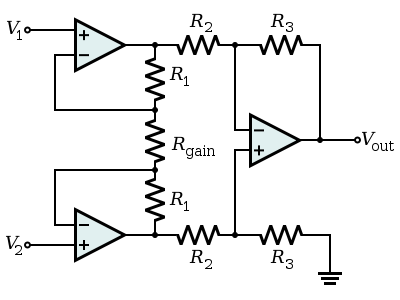
\includegraphics[width=.9\linewidth]{400px-Op-Amp_Instrumentation_Amplifier.svg.png}
\end{frame}
\section{Atmega128A}
\label{sec-3}
\begin{frame}
\frametitle{软件开发环境}
\label{sec-3-1}

\begin{description}
\item[emacs(24.0)] 编辑器
\item[avr-gcc] 编译器
\item[avr-libc] C library for Atmel AVR microcontrollers
\item[avrdude] AVR Downloader
\item[make] Standard tool to compile source trees
\end{description}
\end{frame}
\begin{frame}
\frametitle{ATmega128A 芯片性能概述}
\label{sec-3-2}

High-performance, Low-power Atmel® AVR® 8-bit Microcontroller
\begin{itemize}
\item Up to 16MHz Throughput at 16MIPS
\item 8 channel,10-bit ADC
\item 53 Programmable I/O lines
\item 4Kbytes Internal SRAM
\item SPI Interface for In-System Programming
\end{itemize}
\end{frame}
\begin{frame}
\frametitle{ATmega128A AD性能}
\label{sec-3-3}

\begin{itemize}
\item 10-bit Resolution
\item 0.5 LSB Integral Non-linearity
\item 13 $\mu{}s$ - 260 $\mu{}s$ Conversion Time
\item Sleep Mode Noise Canceler
\item 8 Multiplexed Single Ended Input Channels
\item Interrupt on ADC Conversion Complete
\end{itemize}
\end{frame}
\begin{frame}
\frametitle{AD转换}
\label{sec-3-4}
\begin{itemize}

\item 转换公式 $ADC=\frac{V_{IN}\cdot1024}{V_{REF}}$
\label{sec-3-4-1}%

\item AD寄存器
\label{sec-3-4-2}%

\item 程序中ADCSRA的设置
\label{sec-3-4-3}%
\begin{itemize}
\item $((1 \ll ADEN)|(1 \ll ADIE)|(1 \ll ADPS2)|(1 \ll ADPS1)|(1 \ll ADPS0))$
\item 打开ADC
\item AD转换完成中断打开
\item AD时钟预分频为128
\end{itemize}

\item AD程序
\label{sec-3-4-4}%

\end{itemize} % ends low level
\end{frame}
\begin{frame}
\frametitle{量程切换}
\label{sec-3-5}

\begin{itemize}
\item 中断寄存器
\item 中断程序
\item 具体代码
\item 自动切换量程
\end{itemize}
\end{frame}
\begin{frame}
\frametitle{流程图}
\label{sec-3-6}

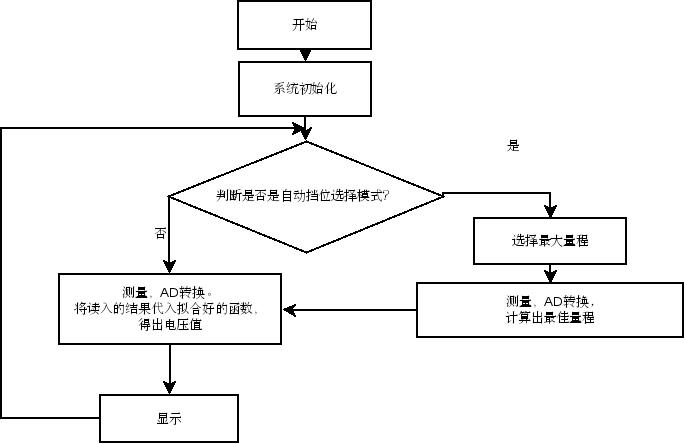
\includegraphics[width=.9\linewidth]{Diagram1.jpg}
\end{frame}
\begin{frame}
\frametitle{0\~{}500mA}
\label{sec-3-7}

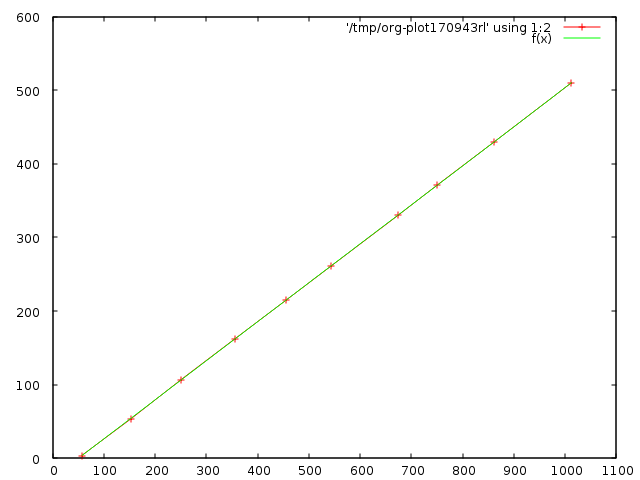
\includegraphics[width=.9\linewidth]{500ma.png}
\end{frame}
\section{LCD12864}
\label{sec-4}
\begin{frame}
\frametitle{性能}
\label{sec-4-1}

\begin{itemize}
\item 性能128x64液晶点阵,8x4中文显示
\item 并行8位数据通行
\item 独立 LED 背光电源
\item 标准 ASCII 字符库和简体中文字库
\end{itemize}
\end{frame}
\begin{frame}[fragile]
\frametitle{单片机和LCD12864通信}
\label{sec-4-2}

\begin{verbatim}
void lcd12864_init(void);
void lcd12864_clear(void);
void lcd12864_move_cur(uint8_t x,uint8_t y);
void lcd12864_write_cmd(uint8_t command);
void lcd12864_write_data(uint8_t wrdata);
\end{verbatim}
\end{frame}
\begin{frame}[fragile]
\frametitle{显示数字和字符串}
\label{sec-4-3}

\begin{verbatim}
void lcd12864_dis_num(int32_t num);
void lcd12864_dis_str(char * str);
\end{verbatim}
\end{frame}
\begin{frame}
\frametitle{显示程序}
\label{sec-4-4}

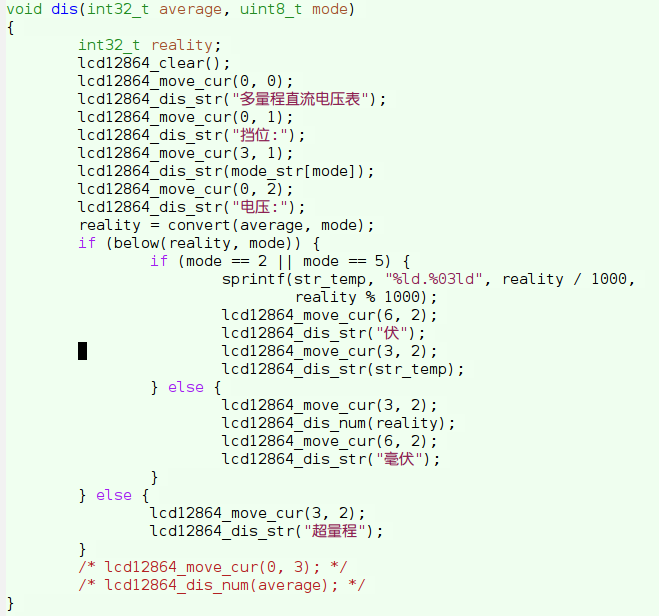
\includegraphics[width=.9\linewidth]{dis.png}

   
\end{frame}

\end{document}